% This is "sig-alternate.tex" V2.0 May 2012
% This file should be compiled with V2.5 of "sig-alternate.cls" May 2012
%
% This example file demonstrates the use of the 'sig-alternate.cls'
% V2.5 LaTeX2e document class file. It is for those submitting
% articles to ACM Conference Proceedings WHO DO NOT WISH TO
% STRICTLY ADHERE TO THE SIGS (PUBS-BOARD-ENDORSED) STYLE.
% The 'sig-alternate.cls' file will produce a similar-looking,
% albeit, 'tighter' paper resulting in, invariably, fewer pages.
%
% ----------------------------------------------------------------------------------------------------------------
% This .tex file (and associated .cls V2.5) produces:
%       1) The Permission Statement
%       2) The Conference (location) Info information
%       3) The Copyright Line with ACM data
%       4) NO page numbers
%
% as against the acm_proc_article-sp.cls file which
% DOES NOT produce 1) thru' 3) above.
%
% Using 'sig-alternate.cls' you have control, however, from within
% the source .tex file, over both the CopyrightYear
% (defaulted to 200X) and the ACM Copyright Data
% (defaulted to X-XXXXX-XX-X/XX/XX).
% e.g.
% \CopyrightYear{2007} will cause 2007 to appear in the copyright line.
% \crdata{0-12345-67-8/90/12} will cause 0-12345-67-8/90/12 to appear in the copyright line.
%
% ---------------------------------------------------------------------------------------------------------------
% This .tex source is an example which *does* use
% the .bib file (from which the .bbl file % is produced).
% REMEMBER HOWEVER: After having produced the .bbl file,
% and prior to final submission, you *NEED* to 'insert'
% your .bbl file into your source .tex file so as to provide
% ONE 'self-contained' source file.
%
% ================= IF YOU HAVE QUESTIONS =======================
% Questions regarding the SIGS styles, SIGS policies and
% procedures, Conferences etc. should be sent to
% Adrienne Griscti (griscti@acm.org)
%
% Technical questions _only_ to
% Gerald Murray (murray@hq.acm.org)
% ===============================================================
%
% For tracking purposes - this is V2.0 - May 2012

\documentclass{sig-alternate}
\usepackage{graphicx,subfigure}

\begin{document}
%
% --- Author Metadata here ---
\conferenceinfo{WWW2015}{Florence, Italy}
%\CopyrightYear{2007} % Allows default copyright year (20XX) to be over-ridden - IF NEED BE.
%\crdata{0-12345-67-8/90/01}  % Allows default copyright data (0-89791-88-6/97/05) to be over-ridden - IF NEED BE.
% --- End of Author Metadata ---

\title{Fact versus Fiction: A Survey of the Varied Use of Untruths Online}

% \subtitle{[Extended Abstract]
%\titlenote{A full version of this paper is available as
%\textit{Author's Guide to Preparing ACM SIG Proceedings Using
%\LaTeX$2_\epsilon$\ and BibTeX} at
%\texttt{www.acm.org/eaddress.htm}}}
%
% You need the command \numberofauthors to handle the 'placement
% and alignment' of the authors beneath the title.
%
% For aesthetic reasons, we recommend 'three authors at a time'
% i.e. three 'name/affiliation blocks' be placed beneath the title.
%
% NOTE: You are NOT restricted in how many 'rows' of
% "name/affiliations" may appear. We just ask that you restrict
% the number of 'columns' to three.
%
% Because of the available 'opening page real-estate'
% we ask you to refrain from putting more than six authors
% (two rows with three columns) beneath the article title.
% More than six makes the first-page appear very cluttered indeed.
%
% Use the \alignauthor commands to handle the names
% and affiliations for an 'aesthetic maximum' of six authors.
% Add names, affiliations, addresses for
% the seventh etc. author(s) as the argument for the
% \additionalauthors command.
% These 'additional authors' will be output/set for you
% without further effort on your part as the last section in
% the body of your article BEFORE References or any Appendices.

\numberofauthors{8} %  in this sample file, there are a *total*
% of EIGHT authors. SIX appear on the 'first-page' (for formatting
% reasons) and the remaining two appear in the \additionalauthors section.
%
% \author{
% You can go ahead and credit any number of authors here,
% e.g. one 'row of three' or two rows (consisting of one row of three
% and a second row of one, two or three).
%
% The command \alignauthor (no curly braces needed) should
% precede each author name, affiliation/snail-mail address and
% e-mail address. Additionally, tag each line of
% affiliation/address with \affaddr, and tag the
% e-mail address with \email.
%
% 1st. author
% 
% all the authors: eMax, DMR, Amy Guy, KMO, LD, DS, Nigel
% \alignauthor
% Author FirstLastName\\
%        \affaddr{Institute for Clarity in Documentation}\\
%        \affaddr{1932 Wallamaloo Lane}\\
%        \affaddr{Wallamaloo, New Zealand}\\
%        \email{trovato@corporation.com}
% % 2nd. author
% \alignauthor
% G.K.M. Tobin\titlenote{The secretary disavows
% any knowledge of this author's actions.}\\
%        \affaddr{Institute for Clarity in Documentation}\\
%        \affaddr{P.O. Box 1212}\\
%        \affaddr{Dublin, Ohio 43017-6221}\\
%        \email{webmaster@marysville-ohio.com}
% % 3rd. author
% \alignauthor Lars Th{\o}rv{\"a}ld\titlenote{This author is the
% one who did all the really hard work.}\\
%        \affaddr{The Th{\o}rv{\"a}ld Group}\\
%        \affaddr{1 Th{\o}rv{\"a}ld Circle}\\
%        \affaddr{Hekla, Iceland}\\
%        \email{larst@affiliation.org}
% \and  % use '\and' if you need 'another row' of author names
% % 4th. author
% \alignauthor Lawrence P. Leipuner\\
%        \affaddr{Brookhaven Laboratories}\\
%        \affaddr{Brookhaven National Lab}\\
%        \affaddr{P.O. Box 5000}\\
%        \email{lleipuner@researchlabs.org}
% % 5th. author
% \alignauthor Sean Fogarty\\
%        \affaddr{NASA Ames Research Center}\\
%        \affaddr{Moffett Field}\\
%        \affaddr{California 94035}\\
%        \email{fogartys@amesres.org}
% % 6th. author
% \alignauthor Charles Palmer\\
%        \affaddr{Palmer Research Laboratories}\\
%        \affaddr{8600 Datapoint Drive}\\
%        \affaddr{San Antonio, Texas 78229}\\
%        \email{cpalmer@prl.com}
% }
\maketitle

\begin{abstract}

\end{abstract}

% A category with the (minimum) three required fields
\category{H.4}{Information Systems Applications}{Miscellaneous}
%A category including the fourth, optional field follows...
\category{D.2.8}{Software Engineering}{Metrics}[complexity measures, performance measures]

% \terms{}

\keywords{Lying online}

\section{Introduction}

% , and has remained the subject of philosophical and theological discussion and debate for centuries~\cite{sanford}

% spectrum ranging from the ordinary connotations associated with deception as a deliberate attempt
% to mislead others to a much larger class of activities that involve portraying information in a way 
% that parts from the full and open representation of understood reality.

Lying and other forms of deception are as fundamental to human interaction as discourse itself, amounting to as much as a third of interpersonal communications by some accounts~\cite{depaulo1996lying}.  By deception, we refer to not only the standard connotation of a deliberate attempt to mislead others, but to a much larger class of activities characterised by the ``any conveyance of information that does not reflect the entirity of known truth''~\cite{camden1984white}.  Deliberately included in such a definition, thus, is the construction of personas or identities meant to represent one's self with attributes different from one's own. 

The benefit of studying such deception in the context of social interaction is that it so often illuminates the ways that people cope with the complexities of the social demands placed on them, within the activities and social contexts they live and work~\cite{camden1984white}.  Online, the use of deception can reveal both the needs and difficulties people have in conducting their interactions and curating their own identities across a large number of online spaces, whilst maintaining their privacy, reputation and roles throughout~\cite{hancock2007digital, Burgoon:2003:TDM:820748.821362}.  

Understanding the use of lying and deception online is important to the Web because so many of the social situations and complexities are either created or profoundly affected by the affordances of the technologies used as the channels fo social interaction themselves \cite{hancock2004deception}.  Technologies that provide new affordances for social interaction, whether simply a new mobile chat app, online forum, or a new communications capability entirely, can fundamentally introduce new social situations and tensions in unanticipated ways.  For example, the immediacy and ubiquity of wireless communications technology is thought to have made commonplace the use of \emph{butler lies}, which are small lies invoked to avoid or take leave of interaction \cite{hancock2009butler} without causing offence.  

In this paper, we present a summary of a survey study in which we sought to characterise the spectrum of lying and deception practices routinely used online.  Rather attempting to at all examine the moral or ethics behind such practices which can be highly subjective and grounded in particular personal philosophies, we seek merely to understand how such deception is used in online settings, and whether such behaviour varies across different social media channels. We find that while there are a wide range of reasons people use deception or identity protection online, few reasons for doing so are malicious (or comprised of ``dark lies''); in fact, a majority of the reasons pertain to impression management, conflict avoidance, and in order to fit in to groups.

In the following sections, we first briefly review the literature on online deception and lying. Second, we briefly describe our methodology and present our results. In the final section, we discuss what we think our findings imply towards the needs pertaining to the web, in particular within the context of the increasing centralisation of social networks and rise of web identity assurance providers.

\section{Background}

% In this section we briefly discuss three sets of related work; first, we discuss a few key studies from social psychology pertaining to lying and deception, followed, second, by an overview of the much smaller literature on deception through computer-mediated communications (CMC) channels, folllwed, in turn, by a description of studies on identity curation, pseudonymous and privacy-preserving behaviours primarily by teens ans other social media users online. 

In \cite{depaulo2003cues}, DePaulo et al. summarise some of historical social psychology literature on lying. In it, they lies are discussed in general classes; \emph{everyday lies} of little consequnce or regret, and \emph{serious lies}, used typically to ``hide transgressions'', ranging from misdeeds to betrayals of trust. Others use the term \emph{white lies} to refer to a class of socially accepted lies, done for a perceived benefit to a social situation or the recipient, while calling the opposite \emph{black lies}, that are generally perceived as the socially or morally reproachable, with \emph{grey lies} existing somewhere in between~\cite{camden1984white}.  In order to characterise the motivations behind lying, Buller and Burgoon derive three categories: \emph{instrumental}, \emph{relational}, pertaining to interpersonal relations, and \emph{identity-related}, pertaining to reputation management~\cite{buller1996testing}. 

Pertaining to online deception, a number of studies have compared online to offline lying practices. Hancock et al.~\cite{hancock2004deception} set out to settle the debate between \emph{media richness theory}, which postulates that lying is more likely in richer interaction (with more and immediate feedback) interactions, against \emph{social distance theory}, which frames lying to be more likely in social cue impoverished settings such as via e-mail, finding support for the latter in their experiments.  Belkin et al. compared lying in e-mail to paper, finding that people were likely to lie on e-mail signficantly more than in personal letters~\cite{naquin2010finer}.  

With respect to experimentation with self-representation, as predicted in Sherry Turkle's seminal work about early digital spaces, \emph{Life on the Screen}~\cite{turkle2011life}, many studies of online studies have confirmed that creating identities .  For example, such studies have revealed frequency with which gamers assume the opposite gender in online play~\cite{hussain2008gender,potts2014love,van2008theorizing}, assume widely different appearances in online virtual environments and massively multiplayer games~\cite{yee2009proteus}, falsify age, height, weight and appearances in online dating sites~\cite{Hancock:2007:TLO:1240624.1240697,JCC4:JCC420}, and experiment with self-representation in on-line chat and discussion spaces~\cite{donath1999identity,whitty2002liar,whitty2001age} to name a few.

Most similar to the work presented in this paper, Caspi et al.~\cite{caspi2006online} conducted a Web survey of Israeli internet users and found that, although a majority of participants believed that deception on the Internet was widespread, only a third ever reported deceiving others online themselves.  Instead of open-ended responses, however their survey asked participants to select among a fixed set of possible personal attributes (age, sex, marital status, height, weight, etc.) and the reasons for doing so. We compare our results to theirs in Discussion.

\section{Method}

We elicited responses via a web-based survey, which we developed from scratch to facilitate use on mobile devices (tablets, phablets and smartphones).  The survey comprised 12 sets of questions including 1 set of demographic questions, and 8 open-answer free responses (see Table \cite{} for a list of questions).  Participant recruitment was done in person at two events in London, at \emph{ComicCon} and the \emph{WebWeWant Festival}, and on-line via Twitter and Facebook.  In person, we distributed a fliers containing the URL to the survey, and posted the URL on visible locations where permitted.  Two popular Internet celebrities, @TheTomSka and @DameWendyDBE helped by posting a link to the survey on their Twitter feeds.

Analysis of free-response questions was done using a \emph{grounded theory} approach; themes were identified across responses through a process starting with open coding procesall open-answer questions by three researchers separately.  Once an initial set of themes for each question was derived, themes were compared between researchers and a final set was derived.  Then, all responses were re-coded against the final set of themes.

\section{Results}

Out of the $N=500$ survey responses, 39\% ($N=198$) provided a gender; 50.2\% responded female, 49.8\% male, and 1\% transgender.  With respect to age, 59\% responded, 91\% were between 18-25, 7\% between 26-35, and 2\% 36+.  We did not expect the age distribution to be so skewed but was likely the result of the young audiences at the two festivals; we discuss the potential implications of this distribution at the end of the paper.

Nearly all respondants were active social media users, although use of particular platforms varied significantly. 

\begin{figure}[ht!]
     \begin{center}
        \subfigure[Facebook]{%
            \label{fig:first}
            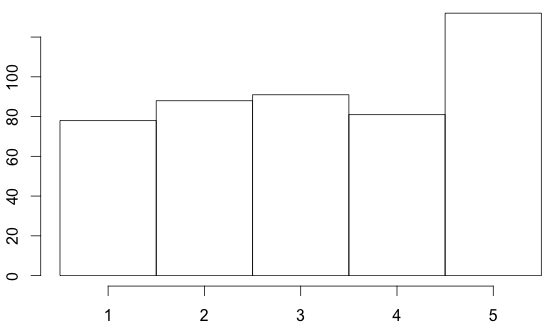
\includegraphics[width=0.24\textwidth]{figs/q1-fb}
        }%
        \subfigure[Twitter]{%
           \label{fig:second}
           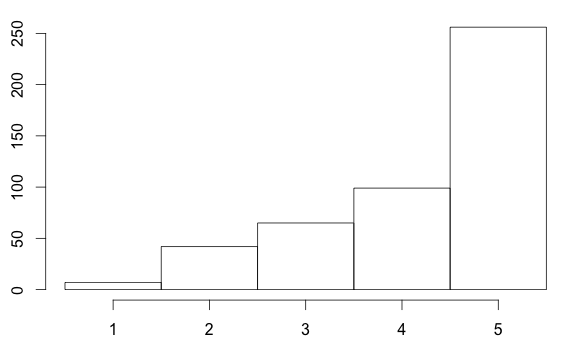
\includegraphics[width=0.24\textwidth]{figs/q1-twitter}
        }\\ %  ------- End of the first row ----------------------%
        \subfigure[Instagram]{%
            \label{fig:third}
            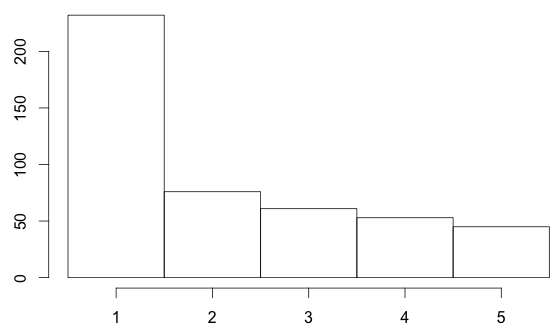
\includegraphics[width=0.24\textwidth]{figs/q1-instagram}
        }%
        \subfigure[Vine]{%
            \label{fig:fourth}
            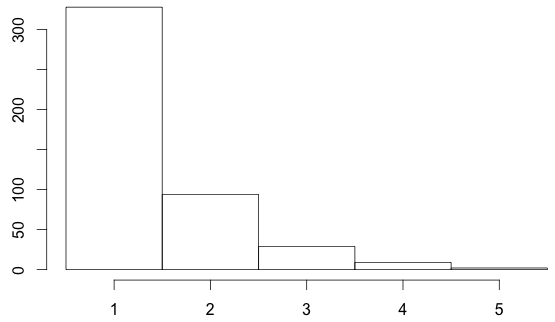
\includegraphics[width=0.24\textwidth]{figs/q1-vine}
        }\\ %
        \subfigure[YouTube]{%
            \label{fig:fifth}
            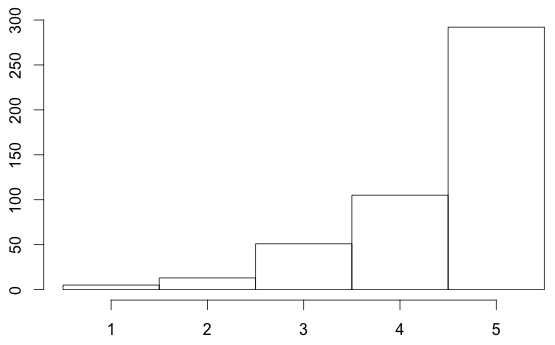
\includegraphics[width=0.24\textwidth]{figs/q1-youtube}
        }%
        \subfigure[Tumblr]{%
            \label{fig:sixth}
            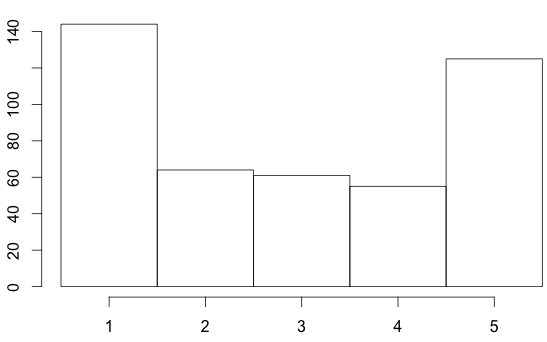
\includegraphics[width=0.24\textwidth]{figs/q1-tumblr}
        }\\ %
    \end{center}
    \caption{%
    	Self-reported use of social media, from 1 = Never to 5 = Several times a day.
     }%
   \label{fig:\texttt{}subfigures}
\end{figure}

\subsection{How much do you lie}
\subsection{Whom }


\section{Discussion}

\section{Limitations}                 
                 
\section{Conclusions}
%\end{document}  % This is where a 'short' article might terminate

\section{Acknowledgments}
%
% The following two commands are all you need in the
% initial runs of your .tex file to
% produce the bibliography for the citations in your paper.
\bibliographystyle{abbrv}
\bibliography{lying-www2015}  % sigproc.bib is the name of the Bibliography in this case
% You must have a proper ".bib" file
%  and remember to run:
% latex bibtex latex latex
% to resolve all references
%
% ACM needs 'a single self-contained file'!
%
%APPENDICES are optional
%\balancecolumns
\end{document}
